\chapter{Présentation de l’organisme d’accueil : CNI}
\label{chap:organisme}

\section{Le Centre National de l’Informatique (CNI)}

Le Centre National de l’Informatique (CNI) est un établissement public à caractère non administratif, doté de la personnalité civile et de l’autonomie financière. Il a été créé le 30 décembre 1975 par la loi n° 75-83 (articles 35 à 42). Placé sous la tutelle du Ministre des Technologies de la Communication, le CNI opère dans les domaines de l’informatique et des technologies de la communication. Il est certifié ISO 9001 version 2015.

\subsection{Missions}

Le CNI constitue le principal appui aux structures publiques de l’administration pour la réalisation, le déploiement et l’exploitation des systèmes d’information. Ses missions couvrent :

\begin{itemize}
\item \textbf{Maîtrise d’ouvrage déléguée} : pilotage de projets.
\item \textbf{Études \& Conseil} : audit, études d’opportunité, schémas directeurs, cahiers des charges, conseils en réseaux et sécurité.
\item \textbf{Développement} : conception, développement et maintenance de systèmes d’information, formation sur les SI développés.
\item \textbf{Hébergement} : hébergement de serveurs, d’applications et de données.
\item \textbf{Backup et continuité d’activité} : mise en place de solutions de reprise après sinistre, élaboration de plans de continuité.
\item \textbf{Formation \& certification} : formations continues, certifiantes, séminaires.
\item \textbf{Déploiement et assistance utilisateurs} : déploiement des applications, assistance sur site ou à distance.
\end{itemize}

\subsection{Historique}

Le CNI a joué un rôle pionnier dans l’informatisation de l’administration tunisienne. Le diagramme ci-dessous résume les grandes étapes de son évolution.

\begin{figure}[H]
\centering
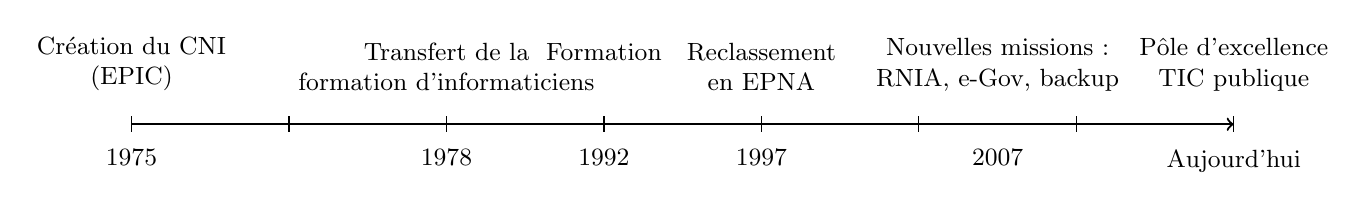
\begin{tikzpicture}[node distance=1.5cm, every node/.style={align=center, font=\small}]
    % Timeline line
    \draw[thick, ->] (0,0) -- (14,0);
    \foreach \x in {0,2,4,6,8,10,12,14}
        \draw (\x,0.1) -- (\x,-0.1);
    
    % Dates and events
    \node[below] at (0,-0.2) {1975};
    \node[above] at (0,0.3) {Création du CNI\\ (EPIC)};
    
    \node[below] at (4,-0.2) {1978};
    \node[above] at (4,0.3) {Transfert de la\\ formation d’informaticiens};
    
    \node[below] at (6,-0.2) {1992};
    \node[above] at (6,0.3) {Formation \\ };
    
    \node[below] at (8,-0.2) {1997};
    \node[above] at (8,0.3) {Reclassement\\ en EPNA};
    
    \node[below] at (11,-0.2) {2007};
    \node[above] at (11,0.3) {Nouvelles missions :\\ RNIA, e-Gov, backup};
    
    \node[below] at (14,-0.2) {Aujourd’hui};
    \node[above] at (14,0.3) {Pôle d’excellence\\ TIC publique};
\end{tikzpicture}
\caption{Chronologie historique du CNI}
\label{fig:historique}
\end{figure}

\subsection{Intégration du projet au sein du CNI}

Le projet XAI-Sleep s’inscrit dans la mission de recherche et développement du CNI, plus particulièrement dans l’axe « Études \& Conseil » et « Développement ». Il répond à une volonté de modernisation des outils d’aide au diagnostic dans le secteur médical, en appliquant les technologies de l’IA explicable aux données de santé. Le CNI m’a offert un environnement favorable, avec un accès à des ressources de calcul et un encadrement de qualité.

\section{Organisation du stage}

Mon stage s’est déroulé sur une période de six mois, du 1er novembre 2024 au 30 avril 2025. Le planning prévisionnel est présenté en annexe. Les principales tâches ont été :

\begin{itemize}
\item Étude de la littérature sur la classification des stades du sommeil et l’IA explicable.
\item Prétraitement des données PSG (Sleep-EDF).
\item Conception et implémentation du modèle d’ensemble (CNN, LSTM, Transformer) avec stacking et LCS.
\item Intégration des méthodes d’explicabilité (SHAP, attention, saliency).
\item Développement d’une API FastAPI et d’une interface web interactive.
\item Mise en place d’une pipeline CI/CD (GitHub Actions, Docker).
\item Évaluation des performances et rédaction du rapport.
\end{itemize}